% !TeX root = ../thesis.tex
\chapter{Background and Motivation: The State of Arithmetic Research Tools}
\label{chp:background}
This chapter sets the stage for the rest of the thesis. It begins by establishing that arithmetic learning in primary school children is an active and relevant research field, then asks what kind of tools that research requires. Six properties of a good research tool are defined and used to evaluate two widely used platforms in the field: OpenSesame and PsychoPy. The chapter closes by examining what happens when these tools fall short, and why the consequences go beyond inconvenience for the researcher.

\section{Arithmetic research in primary school children: an active field}
Most people learn to count before they learn to read, and few skills follow a child further through life than the ability to do arithmetic. Yet despite its seemingly basic nature, how primary school children learn arithmetic remains one of the most actively studied topics in educational psychology. The reason for this is simple: we still do not fully understand how children learn it, why some struggle so much more than others, and what we can do about it.

Part of what makes this field relevant today is that the numbers coming out of large-scale assessments keep raising questions. Belgium's average PISA mathematics score dropped from 508 in 2018 to 489 in 2022, the lowest since the country began participating \cite{globaleconomy2022belgium}, and the trend was already downward before the pandemic (Figure \ref{fig:pisa_scores_belgium}). The same pattern plays out internationally: As the OECD reports, ``mean performance in mathematics across OECD countries fell by a record 15 points'' between 2018 and 2022 \cite{oecd2023pisa}. Something is going wrong, and it is going wrong early.

The stakes are higher than just test scores. As McNeil et al. \cite{ansari2025arithmetic} put it: ``High-quality mathematics education not only improves life outcomes for individuals but also drives innovation and progress across society''. They show that the arithmetic skills a child builds in primary school are not just useful for that year, but they form the foundation for everything that comes after \cite{ansari2025arithmetic}. Early numeracy skills are robust predictors of later mathematical achievement \cite{ansari2025arithmetic}, with strong correlations observed between early assessments and standardized test scores in later years. Children who fall behind in arithmetic early tend to stay behind, and catching up becomes progressively harder as the curriculum moves on \cite{ansari2025arithmetic}.

\begin{figure}
    \centering

    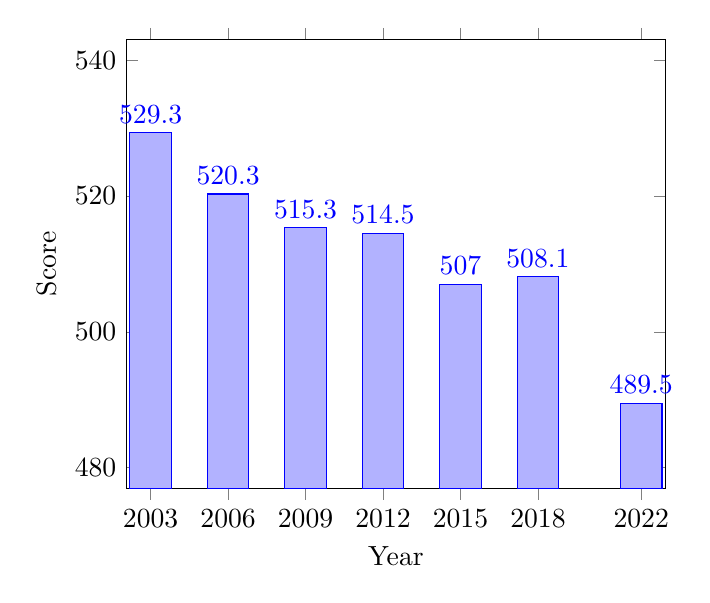
\begin{tikzpicture}
    \begin{axis}[
        xtick=data,
        x tick label style={
            /pgf/number format/1000 sep=},
        xlabel={Year},
        ylabel={Score},
        enlargelimits=0.05,
        ymin=480,
        ymax=540,
        ybar,
        bar width=15pt,
        nodes near coords,
        nodes near coords align={vertical},
    ]

    \addplot coordinates {
        (2003,529.3)
        (2006,520.3)
        (2009,515.3)
        (2012,514.5)
        (2015,507.0)
        (2018,508.1)
        (2022,489.5)
    };

    \end{axis}
    \end{tikzpicture}

    \caption{Evolution of Belgium's PISA mathematics scores from 2003 to 2022, showing a clear downward trend in average performance over time. \cite{globaleconomy2022belgium}}
    \label{fig:pisa_scores_belgium}
\end{figure}

What makes this field particularly active is that arithmetic turns out to be far more complex than it looks from the outside. On the surface, solving a sum seems straightforward. But decades of research have made clear that children bring a whole collection of cognitive skills to the table when they do arithmetic \cite{geary_chapter_2016}. These skills are still developing throughout primary school and that differ substantially from one child to the next. Some of these are specific to numbers: how well children process numerical quantities, or how quickly they retrieve arithmetic facts from memory \cite{vanbinst_chapter_2016}. Others are more general: how well they can hold information in mind \cite{zhang2022working}, how flexibly they switch between strategies \cite{hickendorff2022flexibility}, and perhaps most interestingly, how accurately they judge whether their own answers are correct \cite{rinne_knowing_2014}. De Smedt \cite{desmedt2022} provides an overview of this landscape, noting that individual differences in mathematical performance are remarkably stable and already visible before children enter formal education. Understanding which factors drive these differences, and how they interact across development, remains an open and active research question. 

Researchers at KU Leuven have been prominent contributors to this effort, particularly on the role of metacognitive monitoring in arithmetic achievement \cite{bellon_more_2019, bellon2020, bellon2021} and on individual differences in numerical magnitude processing \cite{vanbinst_chapter_2016}. These are not isolated efforts. Similar questions are being pursued by research groups internationally, each approaching the problem from a different angle \cite{geary_chapter_2016, ansari2025arithmetic, zhang2022working, hickendorff2022flexibility}.

All of this research depends on something practical: tools. Every study in this field depends on being able to observe children doing arithmetic under controlled conditions. Measuring not just whether they get the right answer, but how long it takes, how confident they are, and how their performance evolves over multiple sessions. The quality of that data depends directly on the quality of the tools used to collect it. As this thesis will argue, the tools currently available leave a significant gap between what researchers need and what is currently available. That gap is the starting point for this work.


\section{What a good research tool needs}
\label{sec:research-properties}
Before looking at what is currently available, it is worth being precise about what we are actually looking for. The previous section established that arithmetic research in primary school children is an active field with real scientific stakes. But good research questions can only produce good answers if the tools used to collect the data are up to the job. This section defines what that means in practice.

The six properties described below were developed through a combination of discussions with researchers in the field and a reading of how existing tools are evaluated in the literature on experimental software for educational psychology \cite{peirce_psychopypsychophysics_2007,mathot_opensesame_2012}. They are not claimed to be exhaustive, but together they capture the core requirements that a tool must meet if it is to support rigorous\footnote{In the context of this thesis, ``rigorous'' research is understood in the sense of Shadish, Cook, and Campbell \cite{shadish2002experimental}: research whose design, data collection, and analysis are controlled tightly enough to support valid causal inferences. In practice, this means controlling extraneous variables, collecting complete and accurate data, and producing results that generalise beyond the specific experimental session.}, classroom-based research with children. Each property is introduced and briefly motivated here. The question of how well existing tools satisfy them is taken up in the following section.

\paragraph{Data Tracking}
The most basic requirement of any research tool is that it records what happens. In arithmetic research this means logging not just whether a child answered correctly, but also the response time, the exact answer given, the confidence rating if applicable, and the precise timestamp of each event. Without clean, structured, and complete data, no analysis is possible. This sounds obvious, but in practice many tools either do not log enough detail, make the export process too complex, or produce formats that require preprocessing before they can be used. A good research tool must make data collection automatic, complete, and straightforward to access.

\paragraph{Experimental control}
Research designs in educational psychology typically involve comparing groups under different conditions. For example, children who receive metacognitive prompts versus those who do not. To draw valid conclusions from such a comparison, the researcher must be able to control precisely what each group sees and experiences. This includes controlling the type of exercises presented, the order in which they appear, which items are excluded, whether adaptive difficulty is active or not, and so on. Without this level of control, confounding variables (an outside, often hidden, third variable \cite{salkind2010encyclopedia}) creep in and the internal validity of the study (the extent to which observed effects are caused by the manipulation rather than to other factors \cite{campbell1963experimental}) is compromised.

\paragraph{Reproducibility}
A finding is only scientifically meaningful if it can be replicated. For a tool to support reproducible research, it must be possible to save the complete configuration of an experiment and share it with other researchers so they can run the exact same study. This is closely tied to broader discussions in the open science community about transparency and replication \cite{opensciencecollaboration2015}.

\paragraph{Flexibility}
A research tool is rarely used for a single study. Experiments differ from each other in countless ways, and the same tool needs to support all of them without having to be rebuilt from scratch.

In practice, this means that the parameters a researcher might want to vary need to live outside the source code. This goes beyond simple settings like the number of trials or the timing of how long an item is shown. It also includes structural choices: what kind of stimuli appear (sums, comparisons, word problems, images), how those stimuli are presented and in what order, which prompts the child sees, what counts as feedback, and how a session is organised. If these aspects are hard-coded, the tool does not just become inconvenient to adapt. It becomes impossible for a researcher (or a teacher building their own experiment) to set up the study they actually want. Hard-coded choices turn into real limitations on the study design, which is why flexibility has to be designed in from the start.

\paragraph{Reliability}
Reliability is the property that is easiest to take for granted and most damaging to lose. A research tool is reliable when it behaves the same way for every participant, every session, every time. Timings are accurate (precision), inputs are captured without loss, the interface does not stutter at unpredictable moments (stability), and a crash during session three of a four-session study does not destroy the data from sessions one and two (robustness). None of this is optional. The moment a tool becomes unreliable, the data it produces becomes hard to interpret: ``was that slow response time a real cognitive effect, or was the screen just slow to refresh that trial?'' The concern is not theoretical, millisecond-scale timing errors in commonly used experimental equipment have been documented as a reason for replication failures in reaction-time research \cite{plant2013millisecond}.

Reliability also means working everywhere the study is run, not just on the researcher's development machine. Classroom research typically spans multiple sessions over days or weeks, on hardware the researcher does not control: the school's laptops, the tablets in the library, a mix of browsers on a mix of operating systems. A tool that performs well only under ideal conditions is, for practical purposes, unreliable.

\paragraph{Ease of setup}
A tool can do everything described above perfectly and still be unusable if setting it up takes three weeks and a degree in computer science. The researchers who drive the field are, with few exceptions, not software engineers. If the tool they are meant to use assumes otherwise, there are really only two outcomes: either studies get delayed while someone else writes the experiment, or the study gets reshaped to fit what is easy to implement rather than what the research question actually requires.

Ease of setup is more than the absence of programming. It is the whole experience of getting from ``I want to run this study'' to ``the first child is doing the first exercise.'' Can the researcher tell, by looking at the interface, what each setting does? Is the navigation between configuration screens clear enough that a teacher could manage it during a short training session? When something is misconfigured, does the tool flag the problem before a classroom full of children is already logged in? Visual clarity and guidance through the setup process are what make the difference between a tool a researcher can use independently and one that requires constant developer support.

\section{Current research tools and their limitations}
\label{sec:research-tools}
With a clear picture of what a good research tool needs to do, the next step is to look at what researchers actually have on their desks today. This section walks through the two tools that came up most often during discussions with the research team at KU Leuven: OpenSesame \cite{mathot_opensesame_2012}, a tool frequently used by my co-supervisor in research projects (including the master's thesis discussed in Section \ref{sec:bellon-studies}), and PsychoPy \cite{peirce2019psychopy2}, which is taught to psychology students. The discussion examines how each of them fares against the six properties introduced in Section \ref{sec:research-properties}. Both tools have been carefully designed and have earned their place in the field. The point of this section is not to argue that they are bad tools; it is to show that even the best tools currently available leave a specific kind of gap, and that this gap becomes critical the moment a study leaves the controlled lab and moves into a classroom.

The discussion starts with OpenSesame, then turns to PsychoPy, and ends by drawing out the limitations that both tools share. That final discussion is what motivates the shift in direction taken in Chapter \ref{chp:exercise-tools}.

\subsection{OpenSesame}
Following its authors, OpenSesame is described as ``an open-source, graphical experiment builder for the social sciences'' \cite{mathot_opensesame_2012}. It was designed to make the construction of experiments in the social sciences more accessible than before by providing a graphical user interface (GUI) on top of a Python back-end. A researcher assembles an experiment by dragging items (trial loops, sketchpads, keyboard response components, inline scripts) into a tree structure that represents the flow of the study (as shown in Figure \ref{fig:opensesame_gui}). For anything the GUI does not cover, OpenSesame exposes an inline Python editor that lets the researcher drop directly into code \cite{mathot_opensesame_2012}. It is cross-platform and free.

Against the six properties from Section \ref{sec:research-properties}, OpenSesame scores well on most of them. \textbf{Data tracking} is handled automatically: every trial produces a row in a structured log file, with response times, accuracy, and any custom variables the experimenter defines. \textbf{Experimental control} is one of its strongest points. The researcher has essentially full authority over what each participant sees, the order of stimuli, the exact timing of each event, and the conditions under which the experiment branches. \textbf{Reproducibility} is built into the format: an OpenSesame experiment is stored as a single file that bundles the configuration, the stimuli, and any inline scripts, which means that sharing the experiment with a collaborator is as simple as sharing that file. \textbf{Flexibility} is high because the inline Python escape hatch means there is almost no experimental design the tool cannot, in principle, express. \textbf{Reliability} is more nuanced. Timing precision was measured in an independent benchmark using a hardware Black Box Toolkit, where OpenSesame fell within a 1--5 ms range across visual, audio, and response measures, and performed consistently across Windows, macOS, and Ubuntu \cite{bridges2020timing}. The broader, practical sense of reliability is harder to pin down. Because OpenSesame is a separate software package that has to be installed and configured correctly on each machine, we have heard of cases where it is awkward to get running on classroom hardware. Overall, though, the tool can be considered reliable.

The property where OpenSesame runs into trouble is \textbf{ease of setup}. On the surface, the GUI looks approachable: drag some items, connect them, press run. But the moment the study steps outside the standard kind of experiment where a stimulus is shown and the participant gives a response, the researcher is pulled into Python. Adding a custom adaptive algorithm, implementing a non-trivial exclusion rule, conditionally showing feedback based on the previous answer, or linking trial sequences across multiple sessions: each of these require inline scripts. These scripts are not decoration, they become critical components of the experiment, and maintaining them demands real programming skill. A researcher without a background in Python is effectively stuck with what the GUI alone can do, which for any non-standard arithmetic study is not enough.

\begin{figure}
  \centering
  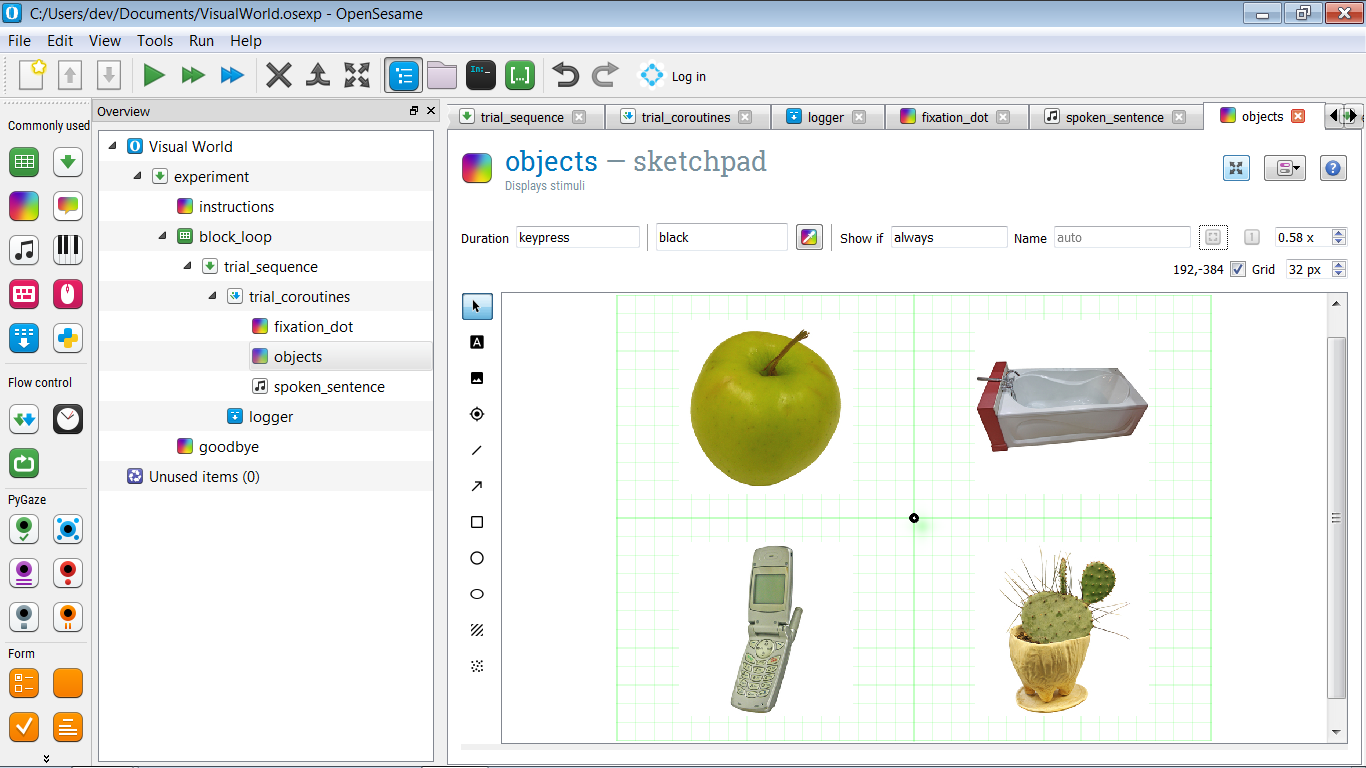
\includegraphics[width=0.85\textwidth]{figures/opensesame_gui.png}
  \caption{Screenshot of the OpenSesame graphical user interface, showing the experiment structure on the left and a sketchpad editor for designing visual stimuli on the right.
  {\cite{mathot_opensesame_2012}}}
  \label{fig:opensesame_gui}
\end{figure}

There is also a second layer to this problem that has little to do with programming. OpenSesame exposes a large number of configuration options across several panels and tabs, with defaults and vocabulary (loops, sketchpads, synchronisation back-ends) that only make sense once the underlying experiment-building model is already familiar. For an experienced user this is manageable, but for someone approaching the tool for the first time the learning curve is steep enough that they will typically need a trained research assistant in the room.

The OpenSesame team continues to develop the project (including a new generative-AI setup assistant \cite{sigmundai} and a web version \cite{mathot2022osweb}), but the underlying picture is unchanged: anything beyond the standard GUI workflow still requires Python. OpenSesame is a powerful tool, but for researchers without a programming background it is limiting.

\subsection{PsychoPy}
PsychoPy is the other open-source tool that comes up frequently in this work. Originally developed by Peirce as a Python library for psychophysics experiments \cite{peirce_psychopypsychophysics_2007}, it has since grown into a full experiment-building environment with its own graphical Builder interface \cite{peirce2019psychopy2}. Where OpenSesame started from the GUI and added Python as an escape hatch, PsychoPy came from the opposite direction: it began as a pure coding library and later wrapped a graphical interface around it. This difference in origin matters because it affects how the tool behaves from a user's perspective.

On the first five properties, PsychoPy performs comparably to OpenSesame. \textbf{Data tracking}, \textbf{experimental control}, \textbf{reproducibility}, and \textbf{flexibility} are all handled at a similar level: logging is automatic and extensible, the researcher has full control over what each participant sees, experiments can be saved and shared as structured files, and the underlying Python library means almost any design can be expressed in code. \textbf{Reliability} is where PsychoPy stands out the most. It was originally developed because existing tools did not offer the timing accuracy that psychophysics research demands \cite{peirce_psychopypsychophysics_2007}, and independent benchmarks confirm that it remains among the most precise lab-based tools available, with mean visual, audio, and response timing under one millisecond \cite{bridges2020timing}. It is also a mature project with a large active community of users and developers \cite{peirce2019psychopy2}, which means bugs tend to be identified and fixed quickly. Like OpenSesame, however, it was designed for controlled lab environments rather than for the hardware mix of a primary school classroom.

That leaves \textbf{ease of setup}, where PsychoPy faces the same fundamental challenge as OpenSesame, but arguably in a more obvious form. The graphical Builder interface offers a drag-and-drop workflow that works well for simple experiments. PsychoPy's own documentation is explicit about the trade-off: the Builder covers standard cases, and for anything more complex the researcher is expected to write raw Python code \cite{peirce2019psychopy2}.

The interface itself reinforces this. A first-time user is confronted with terminology like Routines, Components, Backends, and Monitor configurations: concepts that make sense to someone with a programming background but are not self-evident to a researcher encountering the tool for the first time. The Builder GUI is genuinely well-designed and capable (Figure~\ref{fig:psychopy-ui}), but where OpenSesame attempts to hide the Python layer behind a familiar drag-and-drop tree, PsychoPy keeps it closer to the surface. The result is similar to OpenSesame but shifted further along the technical axis: an excellent tool for a researcher who already knows Python or is willing to learn it, but a steep entry point for anyone else.

\begin{figure}
\centering
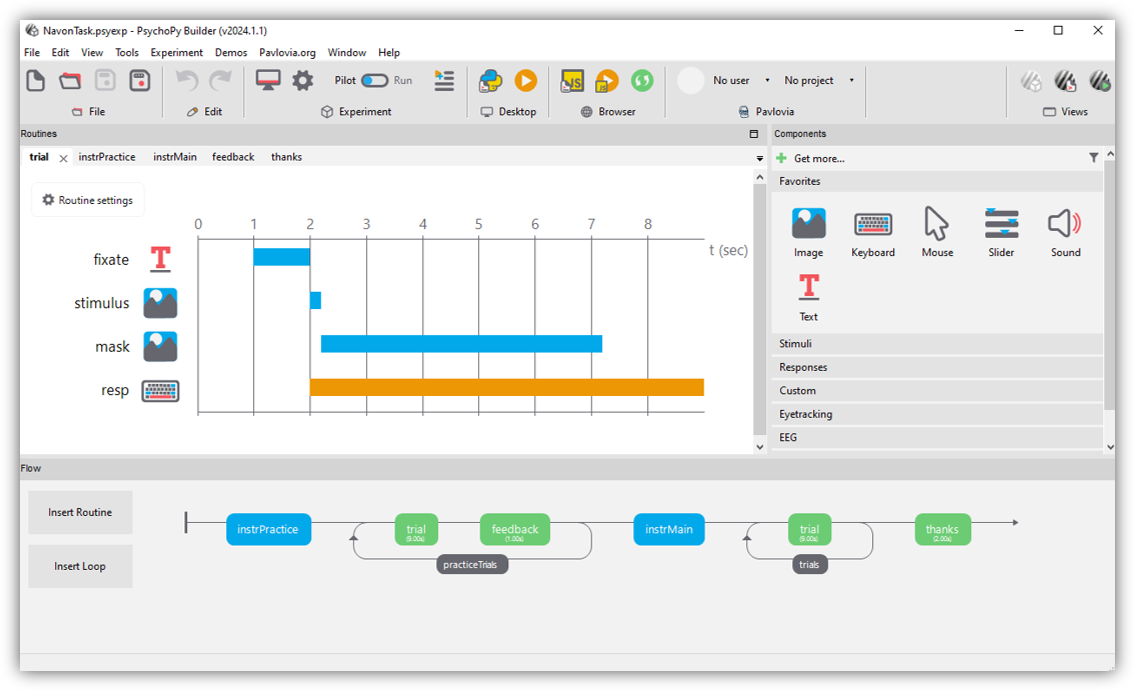
\includegraphics[width=0.85\textwidth]{figures/psychopy_builder.png}
\caption{The PsychoPy Builder interface. Routines are displayed as timelines, and each Component maps onto a set of Python parameters. For experiments that exceed the Builder's built-in Components, researchers insert Code Components containing raw Python, which effectively turns the study into a programming project.}
\label{fig:psychopy-ui}
\end{figure}

At this point, a pattern is becoming visible. Both OpenSesame and PsychoPy satisfy the core research requirements but both run into the same wall when it comes to ease of setup. Figure~\ref{fig:research-tool-grid} summarises this comparison. The six research-tool properties from Section \ref{sec:research-properties} are listed as columns, and each tool is evaluated per property. The first five columns are green; the last one is not. This grid will be extended in Chapter \ref{chp:exercise-tools} when the exercise-tool properties are introduced.

\begin{figure}
\centering
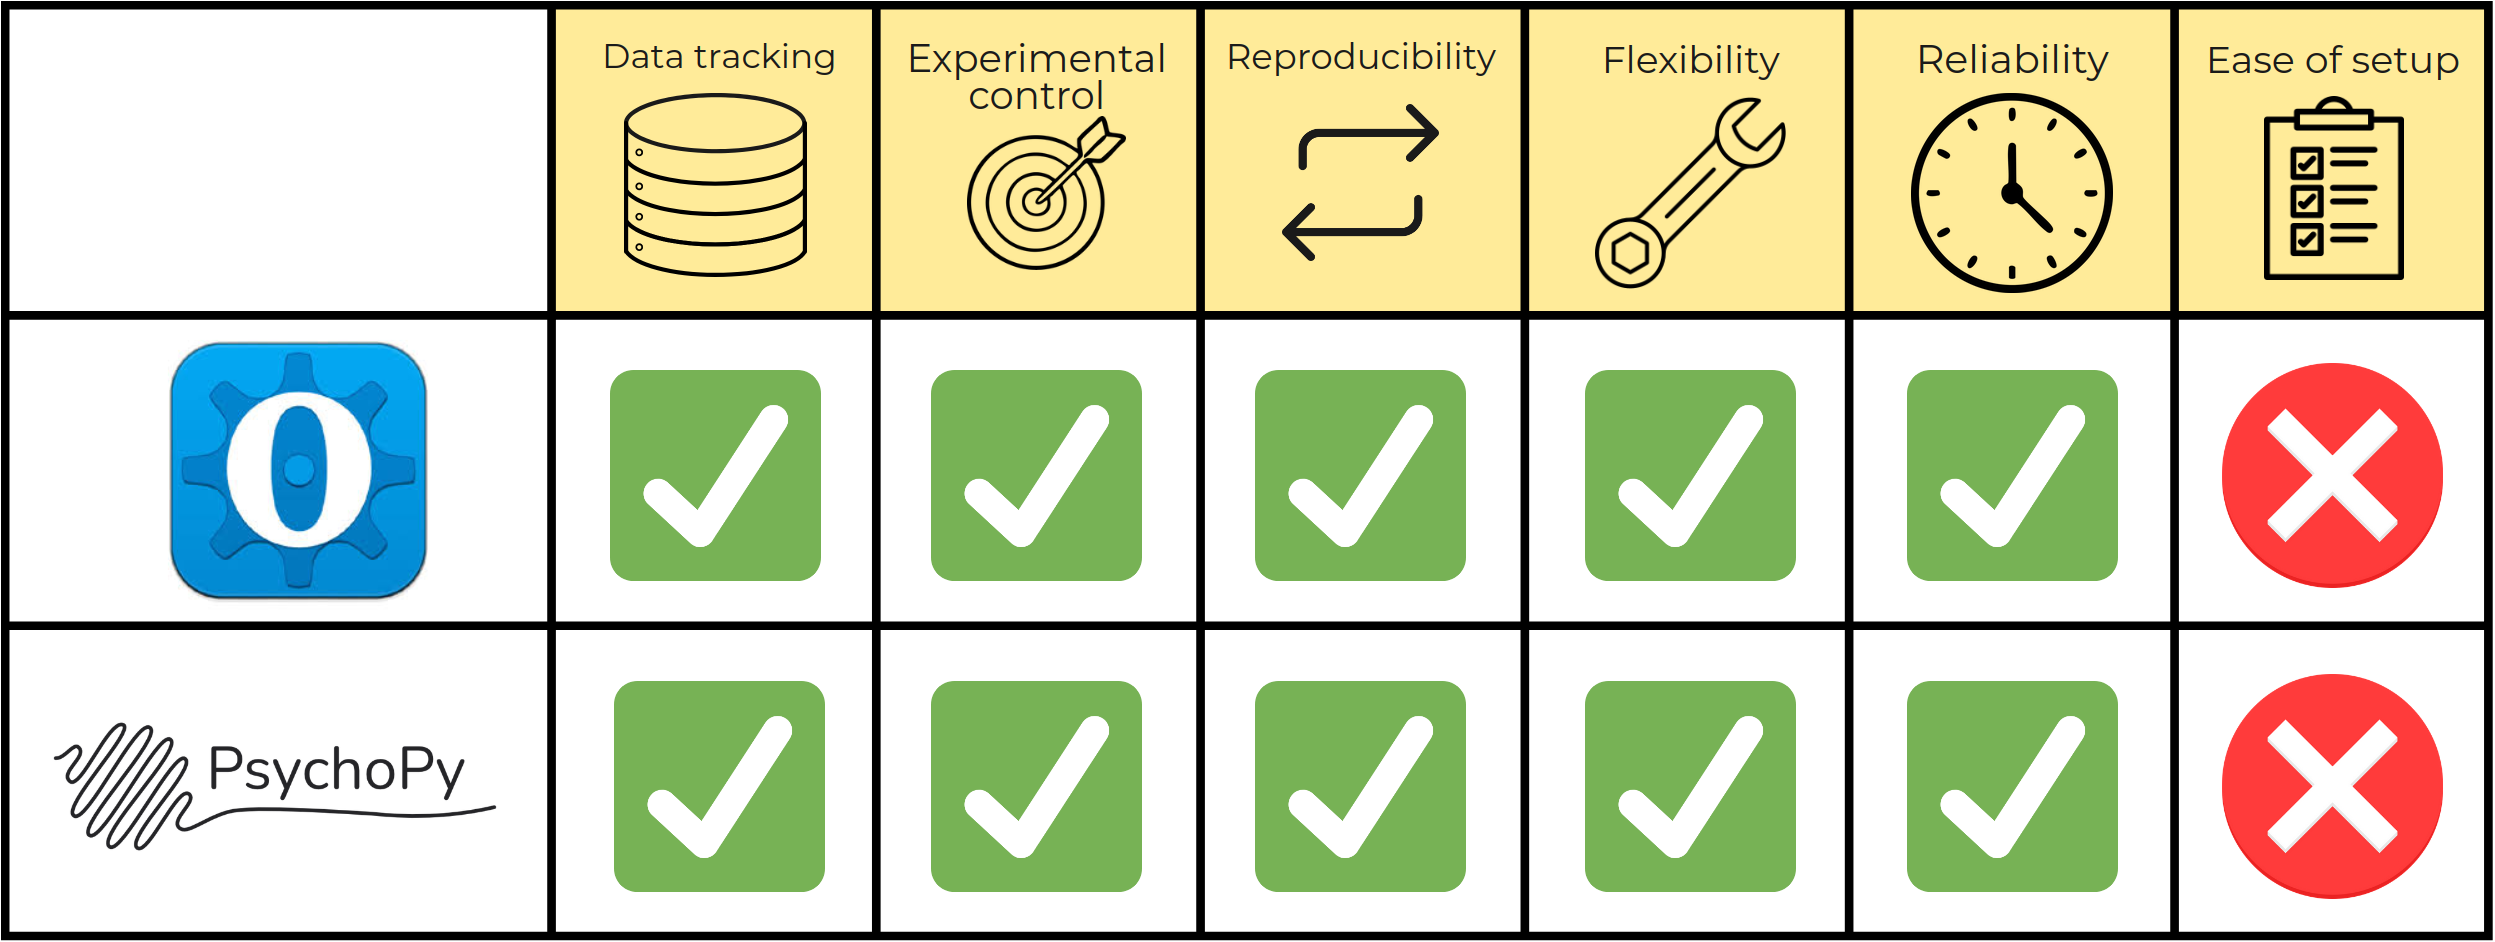
\includegraphics[width=0.85\textwidth]{figures/grid_research_new.png}
\caption{Comparison of OpenSesame and PsychoPy against the six research-tool properties from Section \ref{sec:research-properties}. Both tools satisfy all but the last.}
\label{fig:research-tool-grid}
\end{figure}

\subsection{Shared limitations}
\label{sec:shared-limitations}
The previous sections have shown that OpenSesame and PsychoPy are strong research tools. On five of the six properties defined in Section \ref{sec:research-properties} they deliver exactly what a researcher needs: clean data tracking, full experimental control, reproducible setups, flexible designs, and reliability. But the picture changes completely when you step back and ask a different question: what is it actually like for a child to sit in front of one of these tools?

The answer, in most cases, is that it is not a pleasant experience. A typical arithmetic experiment built in OpenSesame or PsychoPy presents the child with white text on a black screen, one problem at a time, with no story, no colour, no reward, and no sense of progress (see example Figure \ref{fig:black_screen}). There is no character guiding them through the session or puzzle to unlock after ten correct answers. The experiment simply moves from one trial to the next until it is done. For a single short session in a quiet lab, this can work. But arithmetic research often takes place in classrooms, across multiple sessions spread over days or weeks, with children who are seven or eight years old. In that context, a black screen with numbers on it is not enough.

This is not an oversight by the developers of these tools. OpenSesame and PsychoPy were built to be general-purpose experiment builders, and they do that job well. The problem is the one identified in the previous sections: anything beyond the bare stimulus-response loop, gamification, a narrative wrapper, a child-friendly login, has to be built from scratch by the researcher, in Python. Because of the ease-of-setup wall, the researchers who need these features cannot build them. They know exactly what kind of experience they want the child to have, exercises that adapt to the child's level, a colourful interface that feels like a game, metacognitive prompts wrapped in a story. But translating that vision into working code is a skill most of them do not have, and hiring or collaborating with a developer for every study is neither practical nor scalable.

\begin{figure}
\centering
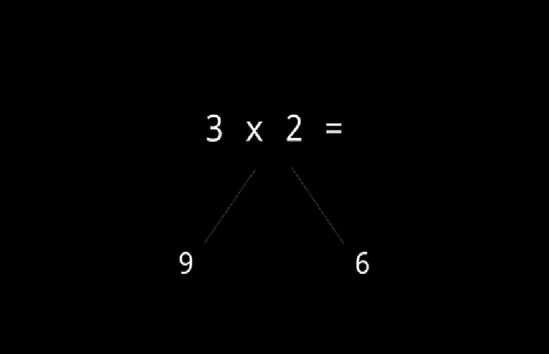
\includegraphics[width=0.65\textwidth]{figures/zwart_scherm.png}
\caption{Example of a stimulus presentation screen created in OpenSesame, showing a simple arithmetic task with multiple-choice response options.}
\label{fig:black_screen}
\end{figure}

This creates a frustrating situation. Researchers who study arithmetic learning in children know their population well. They know what kind of experience would actually serve the child sitting in front of the screen, and how that experience would in turn serve the data they collect. Yet the tools at their disposal make any of that difficult to deliver without significant programming effort. The result is a forced compromise: researchers know what they want, often something that resembles the classroom environment the research is trying to understand, but they cannot deliver it. They end up running studies in conditions stripped of the context they actually care about.

Whether this matters, and how much it matters, is the question taken up in the next section.

\section{Why this matters: the cost of a bad research tool}
\label{sec:why-this-matters}
The limitations described in Section \ref{sec:research-tools} are not just inconveniences for the researcher setting up a study. They have direct consequences for the quality of the research itself. When the tool a child interacts with during an experiment is unfamiliar, visually unappealing, and lacking in motivational features, the data that comes out of that experiment is affected in ways that are hard to control for after the fact. This section discusses three mechanisms through which a poor research tool can compromise a study: reduced ecological validity, motivation drop across sessions, and confounding caused by tool unfamiliarity.

\subsection{Ecological validity}

Ecological validity refers to how well the conditions of a study match the real-world context the research aims to understand \cite{bronfenbrenner1977toward}. Bronfenbrenner argued that studies conducted in artificial laboratory settings, which differ from children's everyday environments, often produce results that are difficult to generalise. Instead, he emphasised the importance of conducting research in natural settings where learning actually occurs, even if these settings are more complex \cite{bronfenbrenner1977toward}.

Shadish, Cook, and Campbell make a similar point in the context of experimental design more broadly: highly controlled lab environments improve internal validity but at the cost of external validity, because the conditions no longer reflect the dynamic nature of real-world learning \cite{shadish2002experimental}.

For arithmetic research with primary school children, this trade-off becomes very concrete. Children today learn arithmetic in environments that adapt to their level, use game-like elements, and let them exercise some control over what they do next. Adaptive difficulty, exercises that get easier or harder based on how the child is doing, keeps learners in a zone where the task is challenging enough to require effort but not so hard that they give up (i.e., zone of proximal development [ZPD]) \cite{murray_zpd_2006}. Adaptive arithmetic learning apps have been shown to improve learning gains and engagement in kindergarten and early primary-school children \cite{bang2023mymathacademy}. Recent systematic reviews have shown that gamification can positively impact the academic performance, motivation, and engagement of primary school children \cite{manzanoleon2021gamification}. A research tool that strips all of these features away does not just produce a less pleasant experience for the child, it produces an experience that no longer resembles the classroom context the research is ultimately trying to study. Whatever is measured under those conditions is, by Bronfenbrenner's definition, less ecologically valid.

\subsection{Motivation drop}
The second cost is more practical and arguably more damaging: children lose motivation. Arithmetic research often spans multiple sessions across days or weeks, and this only works if children stay engaged throughout. Performance on cognitively demanding tasks declines as a function of time on task, and short breaks or changes in activity can partially restore it \cite{sievertsen2016cognitive}. That finding is about fatigue within a single day, but it points to the same underlying issue at the multi-session scale: sustained mental effort produces measurable performance costs, and those costs accumulate when nothing in the task itself works against them.

When the tool itself offers no variation, no rewards, no story, and no sense of progress, the motivation problem is amplified. Research on the role of motivation in mental fatigue has shown that participants who receive motivational incentives are able to maintain performance levels on demanding tasks over extended periods, while those in non-rewarded conditions show clear performance declines \cite{hopstaken2015role}. In the context of arithmetic research with children, this translates to a concrete risk: if the experiment feels boring by session two, the data from sessions three and four may reflect disengagement rather than actual arithmetic ability. The researcher ends up measuring motivation, not mathematics.

The features that could prevent this, gamification, narrative framing, and immediate feedback, are known to support engagement and motivation over time \cite{manzanoleon2021gamification}. They are also precisely the features that most research experiments lack and that the programming barrier described in Section \ref{sec:research-tools} makes difficult to add.

\subsection{The familiarity effect}
The third mechanism is subtler but no less important. When a child encounters a completely unfamiliar tool during a research session, the tool itself becomes a variable in the experiment. The child has to figure out where to type an answer, what the buttons do, how the feedback works, and what is expected of them, all while supposedly demonstrating their arithmetic ability. A related effect is well documented in the testing literature: children tested by a familiar examiner score about 0.28 standard deviations higher than those tested by an unfamiliar one \cite{fuchs1986test}. The same logic plausibly applies to the tool itself: unfamiliarity is a source of irrelevant cognitive load that lowers performance.

If the research tool were also used outside of the experiment, for regular classroom practice or homework, the tool would be invisible during the study in the way a pencil is invisible during a written test: present, but not a source of confusion. The data would more cleanly reflect what the study is actually trying to measure. There is a second advantage too: discoveries made through research, for example that metacognitive prompts improve arithmetic learning, could be fed back into the same tool and reach children as part of their regular practice. The tool would not only serve research but also benefit from it.

\subsection{The bottom line}
All three mechanisms point in the same direction. A research tool that is ecologically valid, motivationally engaging, and familiar to the children who use it is not a luxury or a nice-to-have. It is a prerequisite for producing data that accurately reflects what it claims to measure. In short: a better tool means better research. The question, then, is where to find such a tool. The natural place to look is at the platforms children already use for arithmetic practice in classrooms. That is the direction taken in Chapter \ref{chp:exercise-tools}.

\section{A concrete example}
\label{sec:bellon-studies}
 
The previous section argued, on theoretical and general empirical grounds, that a research tool offering little variation, reward, or sense of progress amplifies the motivation problem across multiple sessions. It is worth grounding that argument in a concrete case. This section looks at one recent master's thesis that ran a multi-session arithmetic training in OpenSesame, the kind of bare stimulus-response setup described in Section~\ref{sec:shared-limitations}. The data from that study are limited, and the patterns described below are at the level of eyeballing rather than formal statistical testing. Still, they offer a concrete illustration of the motivation drop predicted in the previous section.\footnote{The study discussed here is an unpublished master's thesis \cite{baeten2025}. Its results have not undergone peer review, and the patterns reported below should therefore be interpreted with appropriate caution. They are used here as an illustration of a mechanism, not as a definitive empirical claim.}
 
Baeten \cite{baeten2025} studied the relationship between metacognitive monitoring and the arithmetic learning process in 161 third-grade children. To produce a learning process, the children completed a four-day arithmetic training built in OpenSesame, solving the same set of two-digit multiplication exercises once per day across four consecutive school days. Each daily session consisted of 64 items, presented as white text on a black screen with feedback after every answer. This is exactly the type of multi-session, low-engagement experiment that Section~\ref{sec:why-this-matters} identified as being at risk of measuring motivation rather than mathematics.
 
The thesis itself notes this risk. In its discussion of limitations, the author observes that having children complete the same task on four consecutive days can reduce task interest, and that accuracy appeared to stagnate after the second training day rather than continuing to improve \cite{baeten2025}. The thesis also already proposes a partial solution: it suggests that follow-up research could use rewards that depend on the participants' performance, so that children are sufficiently reinforced \cite{baeten2025}. To examine the within-day pattern more closely, the data from the second training day were analysed session by session. Each training day was divided into four successive sessions of sixteen items, and average response time and average accuracy were computed for each session. The result is shown in Figure~\ref{fig:motivation-drop-day2}.
 
\begin{figure}
    \centering
    \begin{subfigure}[t]{0.49\textwidth}
        \centering
        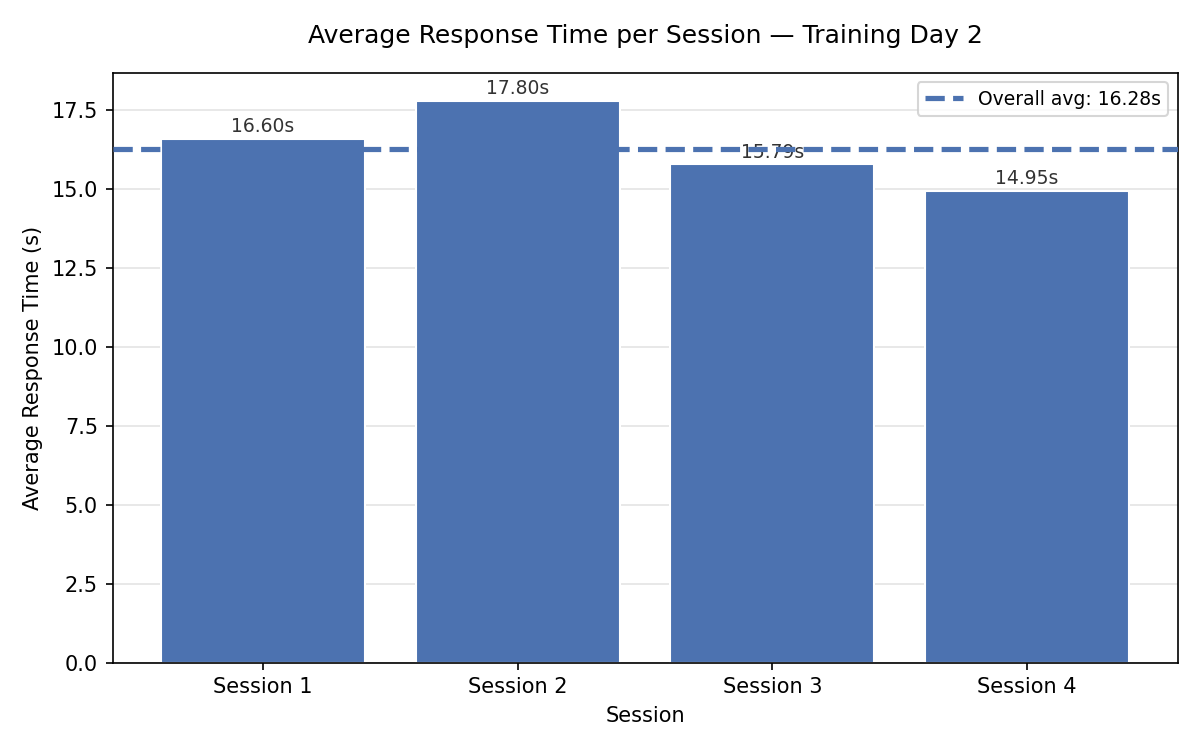
\includegraphics[width=\textwidth]{figures/rt_by_session_day2.png}
        \caption{Average response time per session.}
        \label{fig:rt-day2}
    \end{subfigure}
    \hfill
    \begin{subfigure}[t]{0.49\textwidth}
        \centering
        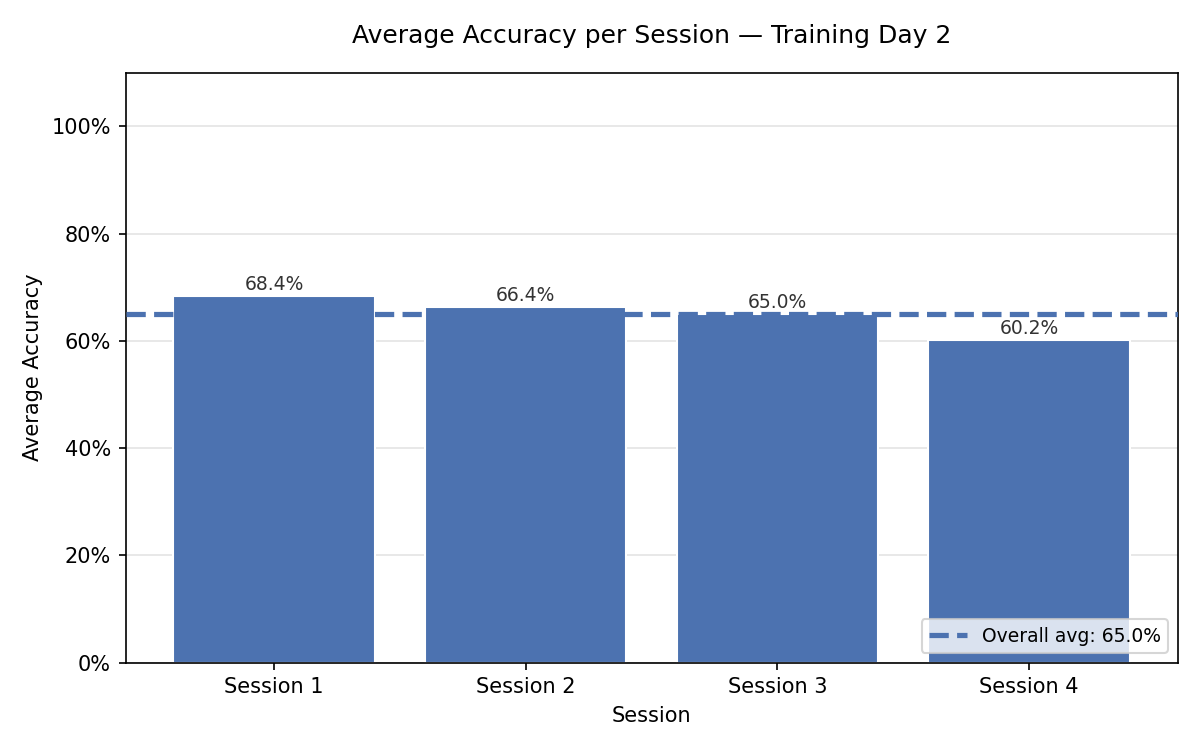
\includegraphics[width=\textwidth]{figures/accuracy_by_session_day2.png}
        \caption{Average accuracy per session.}
        \label{fig:accuracy-day2}
    \end{subfigure}
    \caption{Within-day change across the four sessions of training day~2 in the arithmetic training of Baeten \cite{baeten2025}. As the day progresses, children answer faster while becoming less accurate.}
    \label{fig:motivation-drop-day2}
\end{figure}
 
The two panels point in the same direction. After a small initial rise, the children's average response time falls steadily over the day, from 17.80 seconds in the second session down to 14.95 seconds in the fourth. If this were the only trend, it could be read as a sign of practice or growing fluency. But it is accompanied by the opposite movement in accuracy: the proportion of correct answers drops from 68.4\% in the first session to 60.2\% in the fourth. Children are not getting faster because they are getting better; they are getting faster while getting worse. That combination, shorter response times together with falling accuracy, is consistent with children rushing through the task: clicking quickly to reach the end rather than working through each problem. It appears to be the within-day counterpart of the motivation drop discussed in Section~\ref{sec:why-this-matters}, and it shows up already on the second of four training days.
 
This reading fits what experienced arithmetic researchers report seeing in practice. Bellon (personal communication, 2025) describes three converging signals of waning engagement in this kind of multi-session study. The first is observational: testers notice changes in children's attitude and involvement, such as less task-focused behaviour and less sustained effort. The second is in the behavioural data itself, where disengagement leaves traces such as sudden drops in accuracy, exercises skipped by clicking through quickly, very short response times, and sometimes nonsense answers. The third concerns the learning trajectories: where one would ideally expect gradual progress across training days, that progress is often absent or only weak. The faster-but-less-accurate pattern in Figure~\ref{fig:motivation-drop-day2} is broadly in line with these signals.
 
The lesson here is not that the study was poorly designed. The training was carefully constructed and ran on a capable, widely used research platform, and the thesis itself anticipated the motivation problem and proposed a reward-based fix. The point is rather that delivering such a fix is left entirely to the researcher. A research tool that provided engagement and performance-based rewards by default would lower that barrier, so that addressing the motivation drop does not depend on the individual researcher's programming effort.
 

